\section{Les limites d'ADTool}
	\label{sec:adtool}

	ADTool permet de construire un ADTree sans difficulté. Le logiciel offre la possibilité de créer de nouveaux nœuds, d'éditer leur label et de leur ajouter des fils de façon intuitive et simple. Le choix des opérateurs entre ces nœuds --- conjonction ou disjonction ---  se fait sans effort, et la mise en place de défenses est également réalisable très facilement. 
	
	\begin{figure}[h]
            \centering
            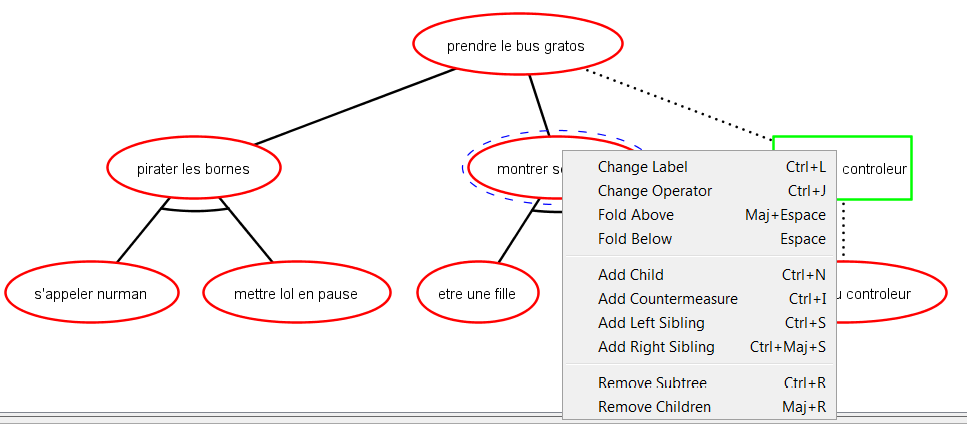
\includegraphics[width=1\textwidth]{figure/not_real_adtool_add_child.png}
            \caption{La création d'un arbre est simplifiée par des fonctions accessibles facilement.}
            \label{fig:arbre_exemple_1}
    \end{figure}
	
	
	Une fois l'arbre établi, il est possible d'ajouter des valuations à chaque feuille\footnote{Une feuille est un nœud n'ayant aucun fils.} de l'arbre selon un paramètre de base, tel que leur coût financier, leur probabilité de réussite, etc. (voir Section \ref{sec::mouloud}). ADTool se charge ensuite de calculer les valuations des nœuds-père de façon récursive, jusqu'à la racine.
	
	\begin{figure}[h]
            \centering
            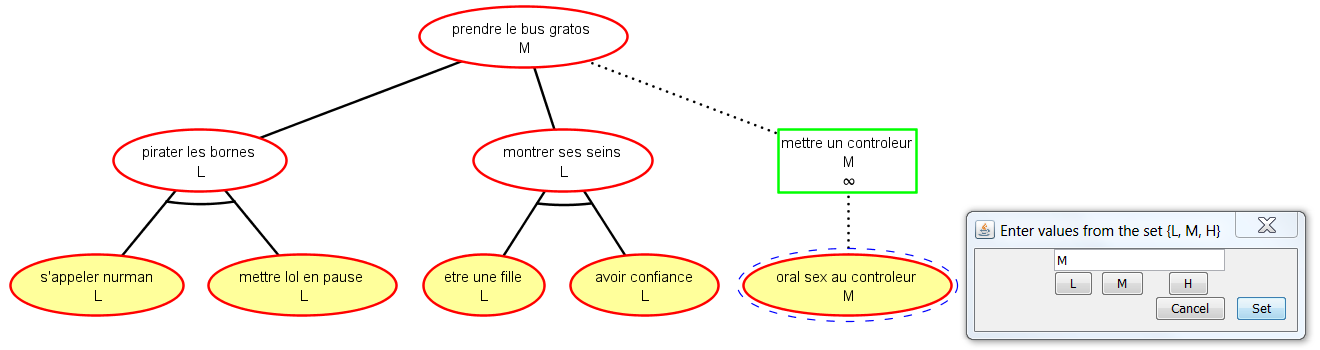
\includegraphics[width=1\textwidth]{figure/not_real_adtool_add_values.png}
            \caption{L'ajout de valuation est simple, et les valuations se propagent récursivement aux nœuds-pères.}
            \label{fig:arbre_exemple_1}
    \end{figure}
	
	Cependant, l'analyse de l'arbre ainsi construit ne va pas plus loin. Les valuations sur chaque noeud ne peuvent se faire que selon un seul paramètre : il n'est par exemple pas possible de prendre en même temps en compte le temps ET le coût d'un nœud. De plus, ADTool ne précise pas d'où provient la valuation d'un nœud donné : par conséquent, pour la racine, l'utilisateur n'a aucun moyen de connaitre l'origine de sa valuation.